% Created 2018-07-24 Tue 17:05
\documentclass[bigger]{beamer}
\usepackage[utf8]{inputenc}
\usepackage[T1]{fontenc}
\usepackage{fixltx2e}
\usepackage{graphicx}
\usepackage{longtable}
\usepackage{float}
\usepackage{wrapfig}
\usepackage{rotating}
\usepackage[normalem]{ulem}
\usepackage{amsmath}
\usepackage{textcomp}
\usepackage{marvosym}
\usepackage{wasysym}
\usepackage{amssymb}
\usepackage{hyperref}
\tolerance=1000
\usepackage{minted}
\usetheme{metropolis}
\author{
\includegraphics[height=0.8cm]{images/Logo_200ok.png} \newline 200ok GmbH}
\date{Alain M. Lafon, 24.07.2018 \newline alain@200ok.ch}
\title{Introduction to ClojureScript and Functional Programming}
\hypersetup{
  pdfkeywords={beamer org orgmode},
  pdfsubject={},
  pdfcreator={Emacs 25.2.2 (Org mode 8.2.10)}}
\begin{document}

\maketitle
\begin{frame}{Outline}
\tableofcontents
\end{frame}


\addtobeamertemplate{frametitle}{}{%
\begin{tikzpicture}[remember picture,overlay]
\node[anchor=north east,yshift=2pt] at (current page.north east) {
\includegraphics[height=0.8cm]{images/Logo_200ok_white.png}};
\end{tikzpicture}}

% Call \framedgraphic with either {filename.jpg} or [size]{filename.jpg}
\newcommand{\framedgraphic}[2][0.7] {
  \center\includegraphics[width=\textwidth,height=#1\textheight,keepaspectratio]{#2}
}

\section{Introduction}
\label{sec-1}

\begin{frame}[label=sec-1-1]{About me}
\begin{columns}
\begin{column}{0.45\textwidth}
\begin{block}{Alain M. Lafon}
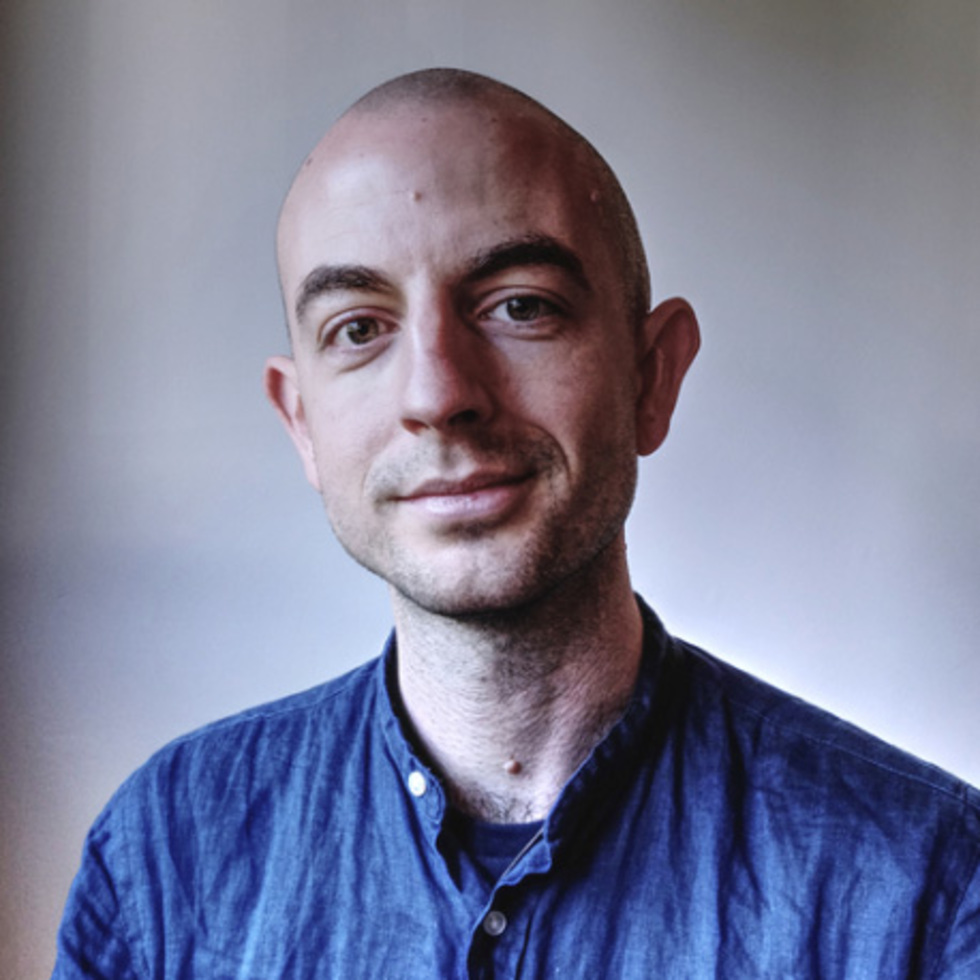
\includegraphics[width=.9\linewidth]{images/alain.jpg}
\end{block}
\end{column}

\begin{column}{0.45\textwidth}
\begin{block}{CV}
\begin{itemize}
\item CEO 200ok GmbH
\item CEO QuickShift GmbH
\item Lecturer at ZHAW
\item Zen Monk, runs the Lambda \href{http://zen-temple.net/zen-temples/lambda-zen-temple/introduction/}{Zen Temple}
\end{itemize}

\begin{block}{Contact}
alain@200ok.ch
\end{block}
\end{block}
\end{column}
\end{columns}
\end{frame}
\begin{frame}[label=sec-1-2]{Questions}
\begin{itemize}
\item I'll cover a lot of ground in this talk
\item However, this is \alert{a lightning talk}
\end{itemize}

\center\rule{0.5\paperwidth}{0.4pt}

\begin{itemize}
\item Please \alert{ask questions} at any time, when something is unclear or
you're simply curious
\end{itemize}
\end{frame}

\begin{frame}[label=sec-1-3]{Before we begin}
\begin{block}{Any LISPers in the room?}
\end{block}
\end{frame}
\begin{frame}[label=sec-1-4]{Right on!}
\framedgraphic{images/gnu_wallpaper.png}
\end{frame}

\begin{frame}[label=sec-1-5]{How did you get started with LISP?}
\begin{itemize}
\item Did some of you start using LISP because of Clojure?
\end{itemize}

\begin{columns}
\begin{column}{0.45\textwidth}
\begin{block}{}
\center
\includegraphics[height=0.25\textheight]{images/clojure_logo.png}
\end{block}
\end{column}

\begin{column}{0.45\textwidth}
\begin{block}{}
\center
\includegraphics[height=0.25\textheight]{images/clojurescript_logo.png}
\end{block}
\end{column}
\end{columns}
\end{frame}


\section{Complexity, Functional Programming and Clojure}
\label{sec-2}

\begin{frame}[label=sec-2-1]{Complexity}
\begin{columns}
\begin{column}{0.45\textwidth}
\begin{block}{}

\begin{itemize}
\item The complexity of software is growing at an exponential rate
\item The biggest problem is the growing complexity of dynamic state which
makes it hard to reason about a system
\end{itemize}
\end{block}
\end{column}


\begin{column}{0.45\textwidth}
\begin{block}{}


\includegraphics[width=.9\linewidth]{images/frp_complexity.png}
\end{block}
\end{column}
\end{columns}
\end{frame}


\begin{frame}[label=sec-2-2]{"State - You're doing it wrong!"}
\begin{center}


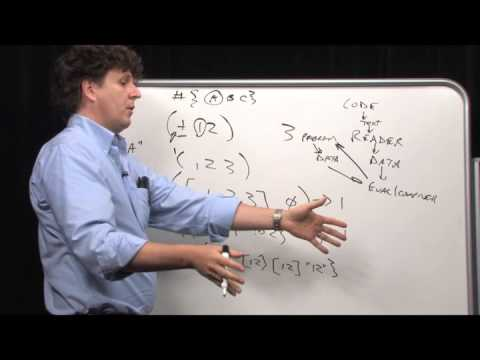
\includegraphics[height=0.6\textheight]{images/rich-hickey.jpg}
\end{center}

Rich Hickey, creator of the Clojure 

Quote Source: \url{http://clojure-log.n01se.net/date/2008-06-26.html#11:10a}
\end{frame}

\begin{frame}[fragile,label=sec-2-3]{Incidental complexity}
 State is hard. And on top, we often use \alert{OOP} and \alert{mutable state} to
make things worse. It is very easy to add incidental complexity to
your application. Just look at this very normal code which probably
doesn't look complex at all:

\begin{minted}[]{javascript}
var x = 1;
var y = x + 1;
y == 2 == true;
x = 2;
y == 3 == false;
\end{minted}

Due to \alert{mutable state}, \texttt{y} was not updated after \texttt{x} has been changed.
This makes reasoning about the current state and logic of the
application hard.
\end{frame}

\begin{frame}[label=sec-2-4]{How to design UI}
\begin{quote}


The UI layer is most predictable when it is described as a pure
function of the application's state.
\end{quote}
\end{frame}

\begin{frame}[label=sec-2-5]{Intro Clojure}
Some of the benefits of Clojure/ClojureScript are:

\begin{itemize}
\item It's a Lisp! (Code as Data)
\item Functional language with immutable persistent data structures
\item Almost no syntax
\item Amazing tooling, Editor integration, performance
\item Use the same language on back-end and front-end
\item Uses Google Closure to optimize your code and included libraries
\item Uncle Bob believes it to be \href{https://skillsmatter.com/skillscasts/2323-bobs-last-language}{the last programming language}
\end{itemize}
\end{frame}

\begin{frame}[fragile,label=sec-2-6]{Syntax Example}
 Syntax example (counting clicks) written in \href{http://reagent-project.github.io/}{Reagent} which builds on
top of \href{https://facebook.github.io/react/}{ReactJS}.

\begin{minted}[]{clojure}
(ns example
  (:require [reagent.core :as r]))
(defonce click-count (r/atom 0))

(defn counting-component []
  [:div
   "Button has been clicked" @click-count " times"
   [:input {:type "button" :value "Click me!"
            :on-click #(swap! click-count inc)}]])
\end{minted}
\end{frame}


\section{Live Demo}
\label{sec-3}

\begin{frame}[label=sec-3-1]{Live Coding - what can go wrong?}
\framedgraphic{images/lambda_workplace.jpg}
\end{frame}


\section{Resources}
\label{sec-4}

\begin{frame}[label=sec-4-1]{Talk tax}
\begin{block}{Slides and minimal example app}
\begin{block}{}
Will be uploaded later to \url{https://200ok.ch}
\end{block}

\begin{columns}
\begin{column}{0.30\textwidth}
\begin{block}{}

\includegraphics[height=0.25\textheight]{images/Logo_200ok.png}
\end{block}
\end{column}


\begin{column}{0.15\textwidth}
\begin{block}{}

\includegraphics[height=0.25\textheight]{images/heart.png}
\end{block}
\end{column}


\begin{column}{0.15\textwidth}
\begin{block}{}

\includegraphics[height=0.25\textheight]{images/clojure_sun.pdf}
\end{block}
\end{column}
\end{columns}
\end{block}
\end{frame}

\begin{frame}[label=sec-4-2]{Watching / Reading List}
\begin{block}{Video}
\begin{itemize}
\item Simple made Easy (Rich Hickey): \url{https://www.infoq.com/presentations/Simple-Made-Easy}
\item Figwheel Demo (Bruce Hauman): \url{https://www.youtube.com/watch?v=KZjFVdU8VLI}
\end{itemize}
\end{block}

\begin{block}{To read}
\begin{itemize}
\item Clojure for the Brave and True: \url{http://www.braveclojure.com/}
\item \url{https://200ok.ch/category/clojure.html}
\item \href{https://200ok.ch/atom.xml}{200ok.ch/atom.xml}
\end{itemize}
\end{block}
\end{frame}

\begin{frame}[label=sec-4-3]{Jobs}
\begin{block}{In case you're searching for a job, talk or write to me!}
\end{block}
\end{frame}


\section{Questions}
\label{sec-5}
% Emacs 25.2.2 (Org mode 8.2.10)
\end{document}
